\section{Discriminating predictions and research program}\label{sec:predictions}

\noindent Table~\ref{tab:predictions} lists \NPred{} predictions, each with a comparison that would weaken the mechanism. P2,
P5, P8, P10, P12, P13, P17, P22, P23, P24, P27 and P34 are the most discriminating against generic demand accounts.

\begin{table*}[tp]
\caption{Discriminating predictions and results that would weaken the mechanism.}
\label{tab:predictions}
\scriptsize
\begin{tabularx}{\textwidth}{@{}P{0.028\textwidth}P{0.19\textwidth}LP{0.25\textwidth}@{}}
\toprule
\# & Prediction & Identifying comparison & Weakening result\\
\midrule
P1 & Information, not endorsement, improves trait judgments & $2\times2$: informative performance $\times$ peer endorsement,
with target, exposure time, and encounters fixed; accuracy on held-out measures & Endorsement raises appeal and confidence
as much as information; no accuracy gain\\
P2 & Diversity beats repetition & Fixed observation time: many domains versus one domain repeated; accuracy for an
independently measured general factor & No advantage, or repetition superior\\
P3 & Choices respond to validity & Information $\times$ measured-ability interaction on consequential choices (Stage~2) &
Uniform appeal gain for all exposed targets\\
P4 & Composites predict reproduction & Field data: composite performance indices versus single domains as predictors of
reproductive success & A single specialized skill dominates\\
P5 & Standing tracks capacity & Natural-fertility populations: correlation $\rho_{ZC}$ between socially assessed standing and
independently measured cognition & $\rho_{ZC}\approx0$ after controls for health and wealth\\
P6 & Assessment is mutual & Both sexes' assessed capacities predict partner quality or reproduction & Strictly one-sided
effects\\
P7 & Kin weigh performance & In arranged-marriage and brideservice systems, kin decisions track observed skill beyond wealth
and alliance & Kin choices ignore observed skill\\
P8 & Decoupling weakens selection & Where heritable material wealth governs access~\cite{borgerhoffmulder2009}, selection on
individually assessed capacity is weaker than in embodied-capital economies & Equal or stronger selection under wealth-based
access\\
P9 & Budget and information steps & Dated brain-size steps follow energetic and information innovations with short lags &
Steps precede innovations by long intervals or are unrelated\\
P10 & Tissue is functionally coupled & Causal designs (within-family, Mendelian randomization) show that brain volume
affects assessed capacity, $a>0$ & $a\approx0$: tissue increase not explained by this mechanism\\
P11 & Leverage is greatest for the least visible traits & Proportional effect of added information is larger for capacities
with low baseline observability ($\sqrt{R_1/R_0}$) & Effects largest for already visible traits\\
P12 & Information at fixed opportunity & Contrasts that change validity while holding the distribution of reproductive
contribution fixed still change the trait--reproduction covariance & Effects appear only when reproductive inequality also
rises\\
P13 & The criterion sets the aim & Standing won by dominance correlates with strength and size; standing conferred as
prestige correlates with independently measured cognition; across societies, more prestige-based standing goes with a larger
$\rho_{ZC}$ & Dominance and prestige standing relate equally, or not at all, to cognition\\
P14 & Safe contests are frequent and informative & Across cultures, contest forms with lower injury rates are held more
often; judgments pooled over many low-stakes bouts predict skill better than a single high-stakes bout & No relation between
severity and frequency; no accuracy gain from pooling\\
P15 & Strong rivals level the group & Across primate groups and human societies, male reproductive skew falls as intergroup
threat rises, controlling for group size & Skew unrelated to threat, or rising with it\\
P16 & Tissue tracks budget, culture tracks network & Across late hominin populations, brain size covaries with markers of
diet quality and fire use, cumulative culture with population connectedness & Brain size tracks network size and not
budget\\
P17 & A floor, not a podium & In natural-fertility populations, selection on men's assessed standing lies mainly in the
access episode (the low tail unpartnered), not in family size among fathers (Eq.~\ref{eq:split}) & Differential concentrated
among fathers at the top\\
P18 & Women's capacities act through survival and help; men's through union duration & Women's measured knowledge and standing
predict child survival and help received more than number of births; men's assessed qualities predict years in union & No
relation to child survival or to union duration\\
\bottomrule
\end{tabularx}
\end{table*}

\begin{table*}[tp]
\caption{Discriminating predictions, continued.}\label{tab:predictionsb}
\scriptsize
\begin{tabularx}{\textwidth}{@{}P{0.028\textwidth}P{0.19\textwidth}LP{0.25\textwidth}@{}}
\toprule
\# & Prediction & Identifying comparison & Weakening result\\
\midrule
P19 & Juries differ & Within one society, partners chosen by kin are selected more on multi-year records of work and
cooperation, self-chosen partners more on short-window cues & Identical criteria\\
P20 & Sign asymmetry in access & Across post-transition populations the access component for men's status is positive; for
women's it is negative where earning and childbearing conflict and moves toward zero or above as they are reconciled; the
number component is negative in both sexes & Same-signed access components in both sexes everywhere\\
P21 & The floor filters load & Burden of rare damaging variants predicts men's childlessness through partnering in
populations beyond the United Kingdom, more strongly in men than women & No sex difference, or no mediation by partnering\\
P22 & Breadth is the target & (a) Holding total excellence fixed, a person competent in several domains is judged higher in
general ability and preferred as a long-term partner or ally over a single-domain specialist; (b) across societies and
species, investment in general capacity rises with the number of domains on which the same individuals are compared, and
falls with division of labor (Propositions~\ref{prop:polymath},~\ref{prop:division}) & Specialists preferred at equal total
excellence; no relation between breadth of common comparison and general capacity\\
P23 & Competence and delivery are complements & Randomized, truthful evidence of reliable investment raises the weight of
competence in consequential partner choices, and evidence of competence raises the weight of reliability
(Proposition~\ref{prop:delivery}); judgments of delivery improve with length of acquaintance more than judgments of capacity
do & A precisely estimated absent or negative interaction; delivery judged as well from first impressions as from long
acquaintance\\
P24 & Staged and unstaged evidence dissociate & Observers given unannounced observation of targets' everyday conduct predict
the targets' later reliability (kept commitments, defaults) better than observers given the same amount of staged
interaction, while the staged observers predict measured ability better (Proposition~\ref{prop:staging}) & No interaction
between kind of evidence and kind of trait, or reliability judged as well from staged interaction\\
P25 & Enforcement shifts the weights & In partner-choice experiments and across societies, the larger the share of a
partner's product whose delivery is guaranteed by third parties, the more choosers weight ability and the less they weight
signs of commitment; evolved or learned generosity is greatest under partial enforcement
(Proposition~\ref{prop:enforce}) & Weights unaffected by enforcement; generosity monotone in enforcement\\
P26 & Breadth taxes exaggeration & An inflated or coached performance in one domain moves judgments of general ability in
proportion to one over the number of domains observed, while a real difference in general ability moves them in full
(Corollary~\ref{cor:inflation}) & The effect of single-domain inflation does not fall with the number of domains\\
P27 & Legibility bounds preference & Randomizing the length of a first encounter (4, 20, 60 minutes) and the number of
observers whose pooled report a chooser sees raises the weight of intelligence and sincerity in choices in step with the
rise in their agreement (Eq.~\ref{eq:sb}), and leaves the weight of looks unchanged or lower (Section~\ref{sec:speed}) &
Weights do not move with length or panel size although agreement does\\
P28 & Who introduces changes what is known & Couples who met through kin, friends or a shared workplace hold more accurate
beliefs about each other's reliability at commitment than couples who met as strangers, with no difference for ability;
couples who met as strangers lengthen the interval before commitment or dissolve early more often
(Proposition~\ref{prop:staging}; Table~\ref{tab:culture}) & No difference by route of meeting in accuracy about
reliability, timing of commitment, or early dissolution, with selection into routes controlled\\
P29 & Selection at the door strengthens for men and appears for women & In cohorts born after 1980, in countries where women's schooling
has overtaken men's, the pairing differential on men's income and schooling keeps rising and women's turns positive, while
the differential among the paired stays near zero for men (Table~\ref{tab:funnel}) & Men's pairing differential falls in
completed cohorts born after 1980\\
P30 & Whoever decides, long observation is what counts & Across societies, the validity of marriage decisions for a
husband's later provisioning and conduct rises with the length of courtship, brideservice or co-residence before marriage,
whether parents or the couple decide (Section~\ref{sec:reschoice}) & No relation between length of prior observation and
later conduct, or a relation only where the couple decide\\
P31 & Firelight adds witnesses & In societies without electric light, reputations for skill and reliability are more
widely agreed among people who share evening gatherings than among those who share only daytime work
(Eq.~\ref{eq:sb}) & Agreement no higher among those who share evenings\\
P32 & A safe contest keeps capacity and loses nerve & Where a dangerous proof of manhood is replaced by a tournament,
ranking in the tournament predicts athletic and foraging capacity as well as the old proof did, and predicts conduct
under real risk less well (Corollary~\ref{cor:ritual}) & Tournament rank predicts conduct under risk as well as the old
proof\\
P33 & A narrow test makes a deficit of a difference & Impairment associated with attention-deficit traits is smaller in
work and schooling that are scored on broad, mobile, self-paced tasks than in seated, sustained, single-task settings, at
equal trait level (Corollary~\ref{cor:narrow}) & Equal impairment across settings\\
P34 & Thin evidence delays unions & Holding age and schooling fixed, people with fewer shared acquaintances at first
meeting take longer to form a co-residential union and more often form none; the interval shortens with the number of
mutual acquaintances (Proposition~\ref{prop:waiting}) & No relation between shared acquaintances and time to union, with
selection into ways of meeting controlled\\
P35 & The shortfall is at the door elsewhere & In other countries with falling births and unchanged ideals, most of the
fall in children per young adult is accounted for by the share never partnered, not by births within unions
(Fig.~\ref{fig:village}B) & Most of the fall arises within unions\\
\bottomrule
\end{tabularx}
\end{table*}

\subsection{Stage 1: information rather than endorsement}

Specify one primary capacity and its measurement model before recording performances, using public-domain batteries such as
the International Cognitive Ability Resource~\cite{condon2014} plus withheld transfer tasks, and estimate reliability in the
recruited sample, because robust experimental tasks can rank individuals poorly~\cite{hedge2018}. Record training,
familiarity, effort, condition, confidence calibration, and socioeconomic opportunity separately; ``drive'' and
``conviction'' are measured, not assumed. The core intervention is a $2\times2$ design crossing access to informative
performance evidence with access to favorable peer endorsement, holding target identity, exposure time, recording quality,
and number of encounters fixed. Information should improve out-of-sample prediction of the measured capacity; endorsement
should not (P1). A further arm compares repeated trials of one task with equally long observation across several domains
(P2), and another compares one high-stakes bout with many low-stakes ones (P14). Targets and stimuli should be modeled as
random factors~\cite{judd2012,westfall2014}.

\subsection{Stage 2: consequential reciprocal choice}

Measure actual voluntary choices (for example, accepting a follow-up conversation) by women and men as both assessors and
targets. The primary estimand is the information $\times$ measured-ability interaction (P3). A uniform increase in appeal for
all exposed targets would indicate familiarity or publicity rather than information. Candidate models of pairing can be
compared with observed couples rather than assuming universal assortative sorting~\cite{conroybeam2021}. We simulated power
for a crossed design in which each target appears in an informative and a matched control condition (Fig.~\ref{fig:power}).
Under the stated assumptions the interaction is small (about \PowSlope{} in choice probability per standard deviation of
ability), and a shared impression from a single recording of each target limits power: with one clip per cell, about
\PowOneLo--\PowOneHi{} targets are needed for 90\% power. Stimulus sampling helps more than adding observers: with four
distinct clips per cell, 400 targets with 40 observers per cell (32,000 decisions) reach \PowFourA\% power and 600 targets
with 20 observers reach \PowFourB\%, where one clip gives \PowOneAtFour\% at 400 targets. These values should be replaced by
pilot estimates in a preregistration that fixes one primary outcome per stage, handles multiplicity, and evaluates prediction
on held-out targets. Participation must be voluntary, data handled securely, and ethics approval obtained; no intervention
should influence reproduction.

\begin{figure}[t]
\centering
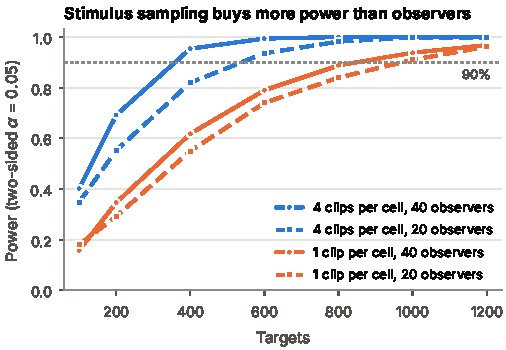
\includegraphics[width=\columnwidth]{figures/figS5_power.pdf}
\caption{\textbf{Simulated power for the Stage-2 information $\times$ ability interaction} (E8; 500 replicates per point).
Assumptions: perceived competence correlates 0.35 with true ability after informative exposure and 0.15 after control
exposure; each clip yields one impression shared by its viewers; choice logit slope 0.8 per SD of perceived competence;
target appeal SD~1; observer intercept SD~0.8; ability measured with reliability 0.8. Analysis: per-target difference in
choice rates regressed on measured ability.}
\label{fig:power}
\end{figure}

\subsection{Stages 3 and 4: field and historical evidence}

Longitudinal and cross-cultural studies in natural-fertility populations should measure $\rho_{ZC}$ (P5) separately for
dominance and prestige (P13), mutual effects (P6), kin decision rules (P7), and the contrast between embodied-capital and
wealth-based economies (P8), testing measurement comparability rather than assuming
it~\cite{vonrueden2016,smith2004,smith2017}. Existing datasets that hold both peer-rated status and cognitive or knowledge
measures, such as the Tsimane studies~\cite{vonrueden2008,vonrueden2011,mcdade2007}, could give a first estimate without new
fieldwork. Historical support requires dated brain-size steps aligned with budget and information innovations (P9), which
the breakpoint intervals of Table~\ref{tab:phases} show to be a weak test at present, and causal evidence that tissue
contributes to capacity (P10). Absence of preserved performance venues is weak evidence, because most performance leaves no
trace.

